\section{Feedback Stimulation Setup}

To elicit electrotactile stimulation in this project the MaxSens stimulation device will be used along with a 16 multi-pad electrode. The following section will provide a short overview of the specification of the stimulation device and electrode. 
 

\subsection{Electrode}

The stimulation 1$\times$16 multi-pad electrode, which is used in this project can be seen on \figref{fig:electrode}, along with dimension information. It is made of 16 circular cathodes, which each share a common long anode. The electrode consists of a polyester layer, an Ag/AgCl conductive layer and a insulation coating. The electrode to skin contact is improved by applying conductive hydrogel pads to the electrode pads. \cite{Strbac2016}     

\begin{figure}[H]                 
	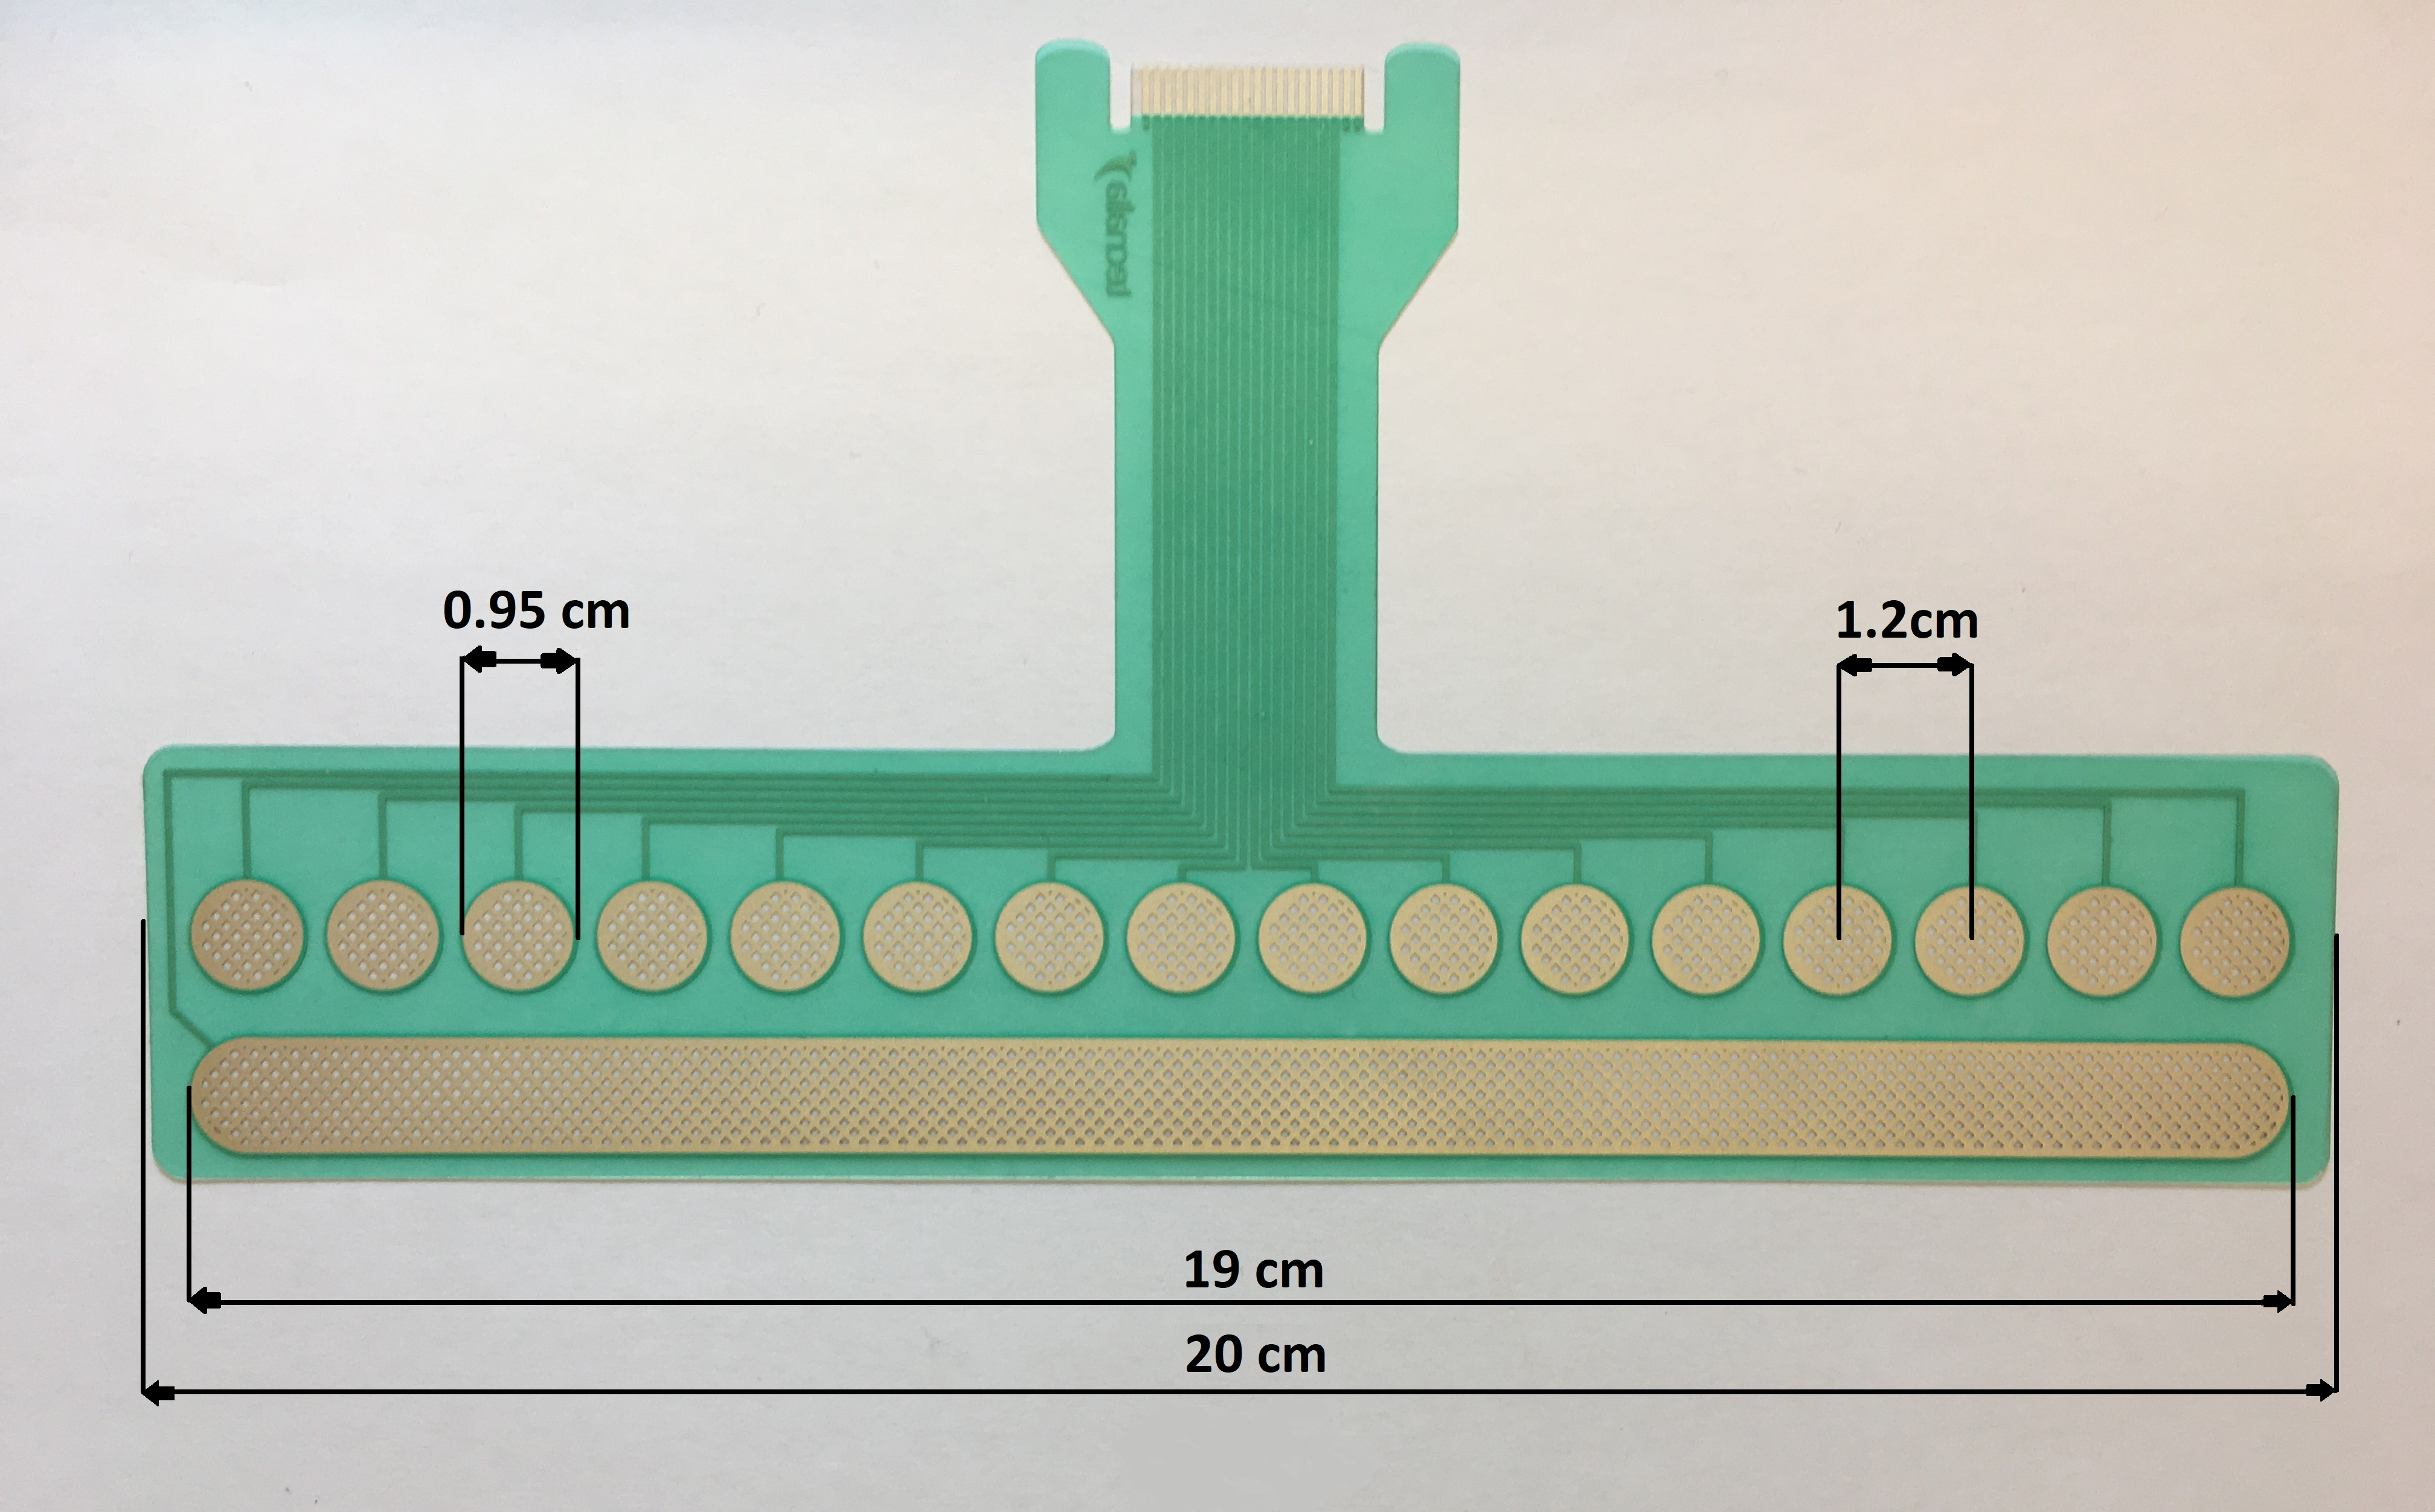
\includegraphics[width=.4\textwidth]{figures/electrode}  
	\caption{The electrode used for electrotactile feedback in this project.}
	\label{fig:electrode} 
\end{figure}


\subsection{MaxSens stimulation device}

The stimulation device is made by MaxSens, Tecnalia, San Sebastian, Spain. Communication between PC and the stimulation device can be achieved either through Bluetooth or a USB connection. The device can be controlled through a series of commands. The MaxSens device allows for independent control of the 16 pads in the electrode. It generates biphasic stimulation pulses where the pulse width can be controlled within a range of 50 $\mu s$ to 1000 $\mu s$ with 10 $\mu s$ steps, pulse rate range of 1 Hz to 400 Hz with 1 Hz steps and current amplitude range of 50 $\mu A$ to 10000 $\mu A$ with 0.1 $\mu A$ steps. Whereas current amplitude and pulse width can be controlled independently for each pad, the pad pulse rate is set globally limiting all pads to have same pulse rate.    